\documentclass[UTF8]{ctexart}
\usepackage{listings}
\usepackage{xcolor}
\usepackage{graphicx}
\usepackage{hyperref}
\usepackage{amsmath}
\usepackage{amssymb}
\usepackage{fontspec}
\usepackage{geometry}
\usepackage{float}
\usepackage{subcaption}
\usepackage[most]{tcolorbox}
\geometry{a4paper, left=2cm, right=2cm, top=2.5cm, bottom=2.5cm}

\definecolor{codegreen}{rgb}{0,0.6,0}
\definecolor{codegray}{rgb}{0.5,0.5,0.5}
\definecolor{codepurple}{rgb}{0.58,0,0.82}
\definecolor{backcolour}{rgb}{0.95,0.95,0.92}

\lstdefinestyle{mystyle}{
    backgroundcolor=\color{backcolour},   
    commentstyle=\color{codegreen},
    keywordstyle=\color{magenta},
    numberstyle=\tiny\color{codegray},
    stringstyle=\color{codepurple},
    basicstyle=\ttfamily\footnotesize,
    breakatwhitespace=false,         
    breaklines=true,                 
    captionpos=b,                    
    keepspaces=true,                 
    numbers=left,                    
    numbersep=5pt,                  
    showspaces=false,                
    showstringspaces=false,
    showtabs=false,                  
    tabsize=2
}

\lstset{style=mystyle}

\title{五子棋游戏技术文档}
\author{Gazettm and pajiiii}
\date{\today}

\begin{document}
\maketitle
\tableofcontents

\section{项目概述}
本项目是一个基于Qt框架的五子棋游戏,支持以下功能:
\begin{itemize}
    \item 双人对战模式
    \item 人机对战模式(AI玩家)
    \item 胜负判定与游戏结束处理
    \item 胜率统计与历史记录
    \item 图形化棋盘界面
\end{itemize}

项目采用MVC架构设计:
\begin{itemize}
    \item \textbf{模型(Model)}: GomokuBoard类管理棋盘状态
    \item \textbf{视图(View)}: GameWindow类处理界面渲染
    \item \textbf{控制器(Controller)}: GameWindow类处理用户输入和游戏逻辑
\end{itemize}

\section{类设计与实现}
\subsection{GomokuBoard类}
棋盘核心逻辑,管理游戏状态。

\subsubsection{成员变量}
\begin{itemize}
    \item \texttt{m\_size}: 棋盘尺寸(默认15×15)
    \item \texttt{m\_board}: 二维向量存储棋子状态
\end{itemize}

\subsubsection{关键方法}
\begin{lstlisting}[language=C++, caption=gomokuboard.h]
enum Piece { Empty, Black, White };
bool placePiece(int x, int y, Piece piece); // 落子
bool checkWin(int x, int y) const;          // 胜负判定
void reset();                               // 重置棋盘
\end{lstlisting}

胜负判定算法:
\begin{lstlisting}[language=C++]
bool GomokuBoard::checkWin(int x, int y) const {
    const int directions[4][2] = {{1,0}, {0,1}, {1,1}, {1,-1}};
    for (auto &dir : directions) {
        int Count = 1;
        // 双向检测连子数量
        for (int i = 1; i < 5; ++i) { // 正向检测
            int nx = x + dir[0] * i, ny = y + dir[1] * i;
            if (nx < 0 || nx >= size() || ny < 0 || ny >= size()) break;
            if (pieceAt(nx, ny) == currentPiece) Count++;
            else break;
        }
        for (int i = 1; i < 5; ++i) { // 反向检测
            int nx = x - dir[0] * i, ny = y - dir[1] * i;
            if (nx < 0 || nx >= size() || ny < 0 || ny >= size()) break;
            if (pieceAt(nx, ny) == currentPiece) Count++;
            else break;
        }
        if(Count >= 5) return true; // 五连珠获胜
    }
    return false;
}
\end{lstlisting}

\subsection{AiPlayer类}
实现AI玩家逻辑,包含位置评估和落子决策。

\subsubsection{核心方法}
\begin{lstlisting}[language=C++, caption=aiplayer.h]
QPoint calculateAIMove(GomokuBoard m_board); // 计算AI落子位置
int evaluatePosition(int x, int y, GomokuBoard::Piece aiPiece, GomokuBoard m_board); // 位置评估
\end{lstlisting}

评估函数实现:
\begin{lstlisting}[language=C++]
int AiPlayer::evaluatePosition(int x, int y, 
    GomokuBoard::Piece aiPiece, GomokuBoard m_board) {
    
    // 防守评分(人类玩家威胁)
    if (humanCount >= 4) score += 100000;   // 阻断四连
    else if (humanCount == 3 && !blocked) score += 10000; // 阻断活三
    
    // 进攻评分(AI连珠)
    if(aiCount == 5) score += 999999;      // 五连绝杀
    else if (aiCount >= 4) score += 5000;   // 四连
    
    // 中心区域加成
    int center = m_board.size() / 2;
    int distance = std::abs(x - center) + std::abs(y - center);
    score += (m_board.size() - distance) * 10;
}
\end{lstlisting}

\subsection{GameWindow类}
主游戏窗口,处理界面和游戏流程。

\subsubsection{游戏流程控制}
\begin{lstlisting}[language=C++]
// 人机对战流程
void GameWindow::mousePressEvent(QMouseEvent *event) {
    if (m_gameMode == HumanVsAI && m_currentPiece != Black) 
        return; // AI回合忽略点击
    
    // 玩家落子
    if (m_board.placePiece(x, y, m_currentPiece)) {
        if (checkWin) ShowWinner(); // 胜负判定
        else {
            m_currentPiece = White; // 切换到AI
            QTimer::singleShot(500, [this]() { // AI延迟落子
                QPoint aiMove = m_aiplayer.calculateAIMove(m_board);
                m_board.placePiece(aiMove.x(), aiMove.y(), White);
                if (checkWin) ShowWinner();
                else m_currentPiece = Black; // 切回玩家
            });
        }
    }
}
\end{lstlisting}

\subsection{Rating类}
胜率统计系统,基于文件存储历史记录。

\subsubsection{核心方法}
\begin{lstlisting}[language=C++]
Rating::Rating(): rating(0), Y(0), N(0){
	std::string filename = "Rating.txt";
	std::ifstream file(filename);
	if (!file) {
		std::ofstream createFile(filename);
		if (createFile) {
			createFile.close();
			file.open(filename);
		}
	}
	std::string line;
	while (std::getline(file, line)) {
		if(line[0] == 'Y')Y++;
		if(line[0] == 'N')N++;
	}
	file.close();
	if (N == 0 && Y == 0) {
		rating = 0;
		message = QString("无信息");
		return;
	} else if (Y == 0) {
		rating = 0;
	} else if (N == 0) {
		rating = 100;
	} else {
		rating = Y / (Y + N) * 100;
	}
	message = QString("您的人机对战胜率为 %1 %").arg(rating, 0, 'f', 2);
}

void Rating::ShowRating(){
	QMessageBox msgBox;
	msgBox.setWindowTitle("胜率");
	msgBox.setText(QString("%1\nYes确认,No清空胜率").arg(message));
	msgBox.setStandardButtons(QMessageBox::Yes | QMessageBox::No);
	msgBox.setDefaultButton(QMessageBox::Yes);
	int ret = msgBox.exec();
	if (ret == QMessageBox::No) {
		std::ofstream file("Rating.txt", std::ios::trunc);
		if (!file) {
			return;
		}
		file.close();
	}
}
\end{lstlisting}
\subsubsection{数据结构}
\begin{itemize}
    \item \texttt{rating}: 胜率百分比
    \item \texttt{Y}: 胜利次数
    \item \texttt{N}: 失败次数
    \item \texttt{message}: 胜率显示信息
\end{itemize}

\subsubsection{文件存储格式}
\begin{lstlisting}
Y  // 人类玩家获胜记录
N  // AI获胜记录
\end{lstlisting}

\section{关键算法}
\subsection{AI评估算法}
采用基于规则的评估函数,考虑因素:
\begin{enumerate}
    \item \textbf{防守优先级}:优先阻断对手四连(100000分)
    \item \textbf{进攻机会}:构建自身连珠(优先构建五连999999分)
    \item \textbf{位置价值}:中心区域权重更高
\end{enumerate}

评分权重矩阵:
\[
\text{Score} = \sum_{\text{方向}} \begin{cases} 
100000 & \text{对手4连} \\
10000 & \text{对手活3} \\
5000 & \text{AI活3/4连} \\
500 & \text{AI活2}
\end{cases} + 10 \times (n - |x - c| - |y - c|)
\]

\subsection{胜率统计算法}
\[
\text{胜率} = \frac{Y}{Y + N} \times 100\%
\]
\begin{itemize}
    \item $Y$:从Rating.txt读取的"Y"行数
    \item $N$:从Rating.txt读取的"N"行数
\end{itemize}

\section{用户界面设计}
界面组件与功能:
\begin{itemize}
    \item \textbf{模式选择对话框}:游戏启动时选择人机/双人模式
    \item \textbf{棋盘绘制}:使用QPainter绘制15×15网格
    \item \textbf{棋子渲染}:黑色实心圆(玩家),白色空心圆(AI)
    \item \textbf{胜率对话框}:显示历史胜率并提供清空选项
    \item \textbf{获胜提示}:模态对话框显示获胜方
\end{itemize}

界面操作流程:
\begin{enumerate}
    \item 启动游戏 → 选择对战模式
    \item 显示历史胜率(可选择清空)
    \item 玩家点击落子(人机模式下AI自动响应)
    \item 五连珠时显示获胜对话框
    \item 游戏结束记录胜率
\end{enumerate}
\section{测试}
\subsection{图片展示}
\begin{figure}[htbp]
    \centering
    \begin{subfigure}[b]{0.3\textwidth}
        \centering
        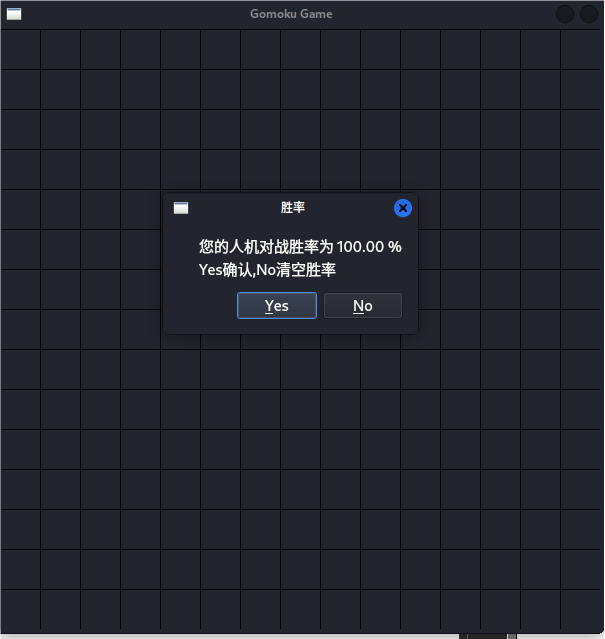
\includegraphics[width=\textwidth]{screenshoot1.png}
        \caption{图1}
        \label{fig:image1}
    \end{subfigure}%
    \hfill
    \begin{subfigure}[b]{0.3\textwidth}
        \centering
        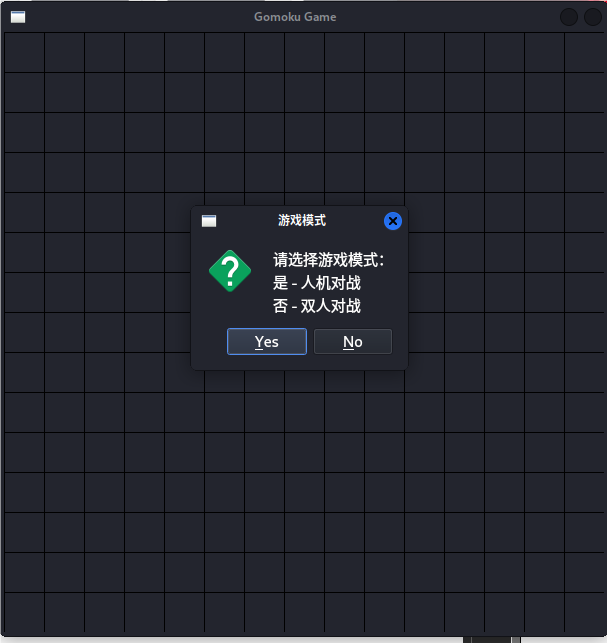
\includegraphics[width=\textwidth]{screenshoot2.png}
        \caption{图2}
        \label{fig:image2}
    \end{subfigure}%
    \hfill
    \begin{subfigure}[b]{0.3\textwidth}
        \centering
        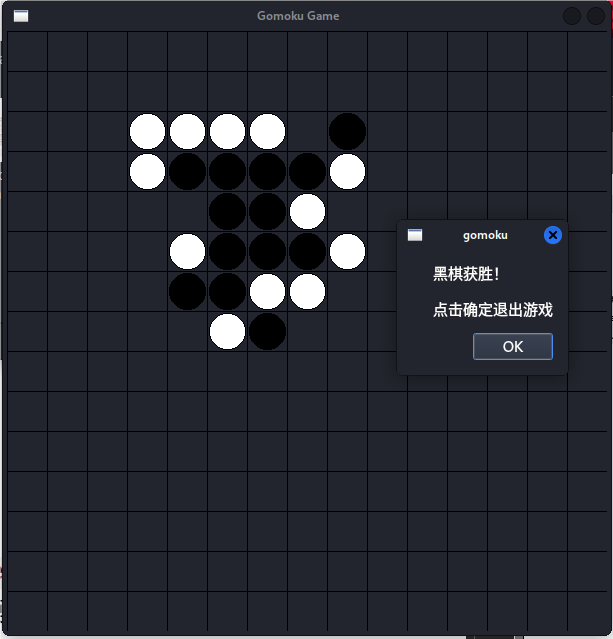
\includegraphics[width=\textwidth]{screenshoot3.png}
        \caption{图3}
        \label{fig:image3}
    \end{subfigure}
    \caption{测试图例}
    \label{fig:allimages}
\end{figure}
\subsection{版本说明}
\begin{itemize}
    \item May 14, 2025 测试
    \item May 24, 2025 linux下texmaker测试(使用xelatex)
    \item May 27, 2025 添加AI
    \item May 28, 2025 优化判定算法
    \item May 31, 2025 添加胜率
    \item Jun 1, 2025 修复bug
\end{itemize}
\section{编译运行说明}
\subsection{环境要求}
\begin{itemize}
    \item Qt 5.15.15
    \item c++ (Debian 14.2.0-19) 14.2.0
    \item g++ (Debian 14.2.0-19) 14.2.0
\end{itemize}

\subsection{编译步骤}
\begin{enumerate}
    \item 编译项目(提前写的makefile文件):
\begin{lstlisting}[language=bash]
CXX = g++
CXXFLAGS = -std=c++11 -Wall -fPIC
QT_INCLUDE = -I/usr/include/x86_64-linux-gnu/qt5/ \
             -I/usr/include/x86_64-linux-gnu/qt5/QtWidgets \
             -I/usr/include/x86_64-linux-gnu/qt5/QtGui \
             -I/usr/include/x86_64-linux-gnu/qt5/QtCore
QT_LIBS = -lQt5Widgets -lQt5Gui -lQt5Core

SRC = main.cpp gamewindow.cpp gomokuboard.cpp aiplayer.cpp Rating.cpp
OBJ = $(SRC:.cpp=.o) moc_gamewindow.o  # 添加 moc 生成的目标文件
TARGET = gomoku

all: $(TARGET)

$(TARGET): $(OBJ)
	$(CXX) $(CXXFLAGS) $^ -o $@ $(QT_LIBS)

# 生成 moc 文件
moc_%.cpp: %.h
	moc $< -o $@

# 编译 moc 文件
moc_%.o: moc_%.cpp
	$(CXX) $(CXXFLAGS) $(QT_INCLUDE) -c $< -o $@

# 编译普通源文件
%.o: %.cpp
	$(CXX) $(CXXFLAGS) $(QT_INCLUDE) -c $< -o $@

clean:
	rm -f $(OBJ) $(TARGET) moc_*
\end{lstlisting}
\item 写makefile文件:
\begin{lstlisting}[language=make]
make
\end{lstlisting}
    \item 运行程序:
\begin{lstlisting}[language=bash]
./gomoku
\end{lstlisting}
\end{enumerate}s

\subsection{文件说明}
\begin{tabular}{|l|l|}
\hline
\textbf{文件} & \textbf{功能} \\
\hline
gamewindow.cpp & 主窗口和游戏流程控制 \\
gomokuboard.cpp & 棋盘状态管理和规则逻辑 \\
aiplayer.cpp & AI玩家决策算法 \\
rating.cpp & 胜率统计系统 \\
main.cpp & 程序入口点 \\
Rating.txt & 胜率数据存储 \\
\hline
\end{tabular}
\section{分工}
Gazettm:
\begin{itemize}
	\item gomokuboard
    \item gamewindows
    \item aiplayer
    \item Makefile
    \item LaTex
\end{itemize}
\medskip
pajiiii:
\begin{itemize}
	\item aiplayer
	\item PPT
	\item markdown
	\item Rating
\end{itemize}

\end{document}